\documentclass{article}
\usepackage[utf8]{inputenc}
\usepackage[a4paper, total={6in, 9in}]{geometry}
\usepackage[francais]{babel}
\usepackage{natbib}
\usepackage{graphicx, caption, float}
\usepackage{listings, lstautogobble}

\setlength{\parindent}{0pt}
\newcommand{\HRule}{\rule{\linewidth}{0.5mm}}

\begin{document}


\begin{titlepage}
\begin{center}


\textsc{\LARGE \'Ecole Polytechnique Fédérale de Lausanne}


\includegraphics[width=0.3\textwidth]{EPFL_logo.jpg}~\\[5cm]
% Title

{ \huge \bfseries Databases Project \\[0.4cm] }

\HRule \\[0.4cm]

{ \huge \emph{First and Second deliverable} \\[6cm] }

% Author and supervisor
\noindent
\begin{minipage}{0.4\textwidth}
\begin{center} \large
\emph{Authors:}\\
Valentine \textsc{Arrieta}\\
Morgan \textsc{Bruhin}\\
Tristan \textsc{Overney}

\end{center}
\end{minipage}%


\vfill

% Bottom of the page
{\large \today}

\end{center}
\end{titlepage}

\section{First deliverable}
\subsection{ER model}

    \begin{figure}[H]
        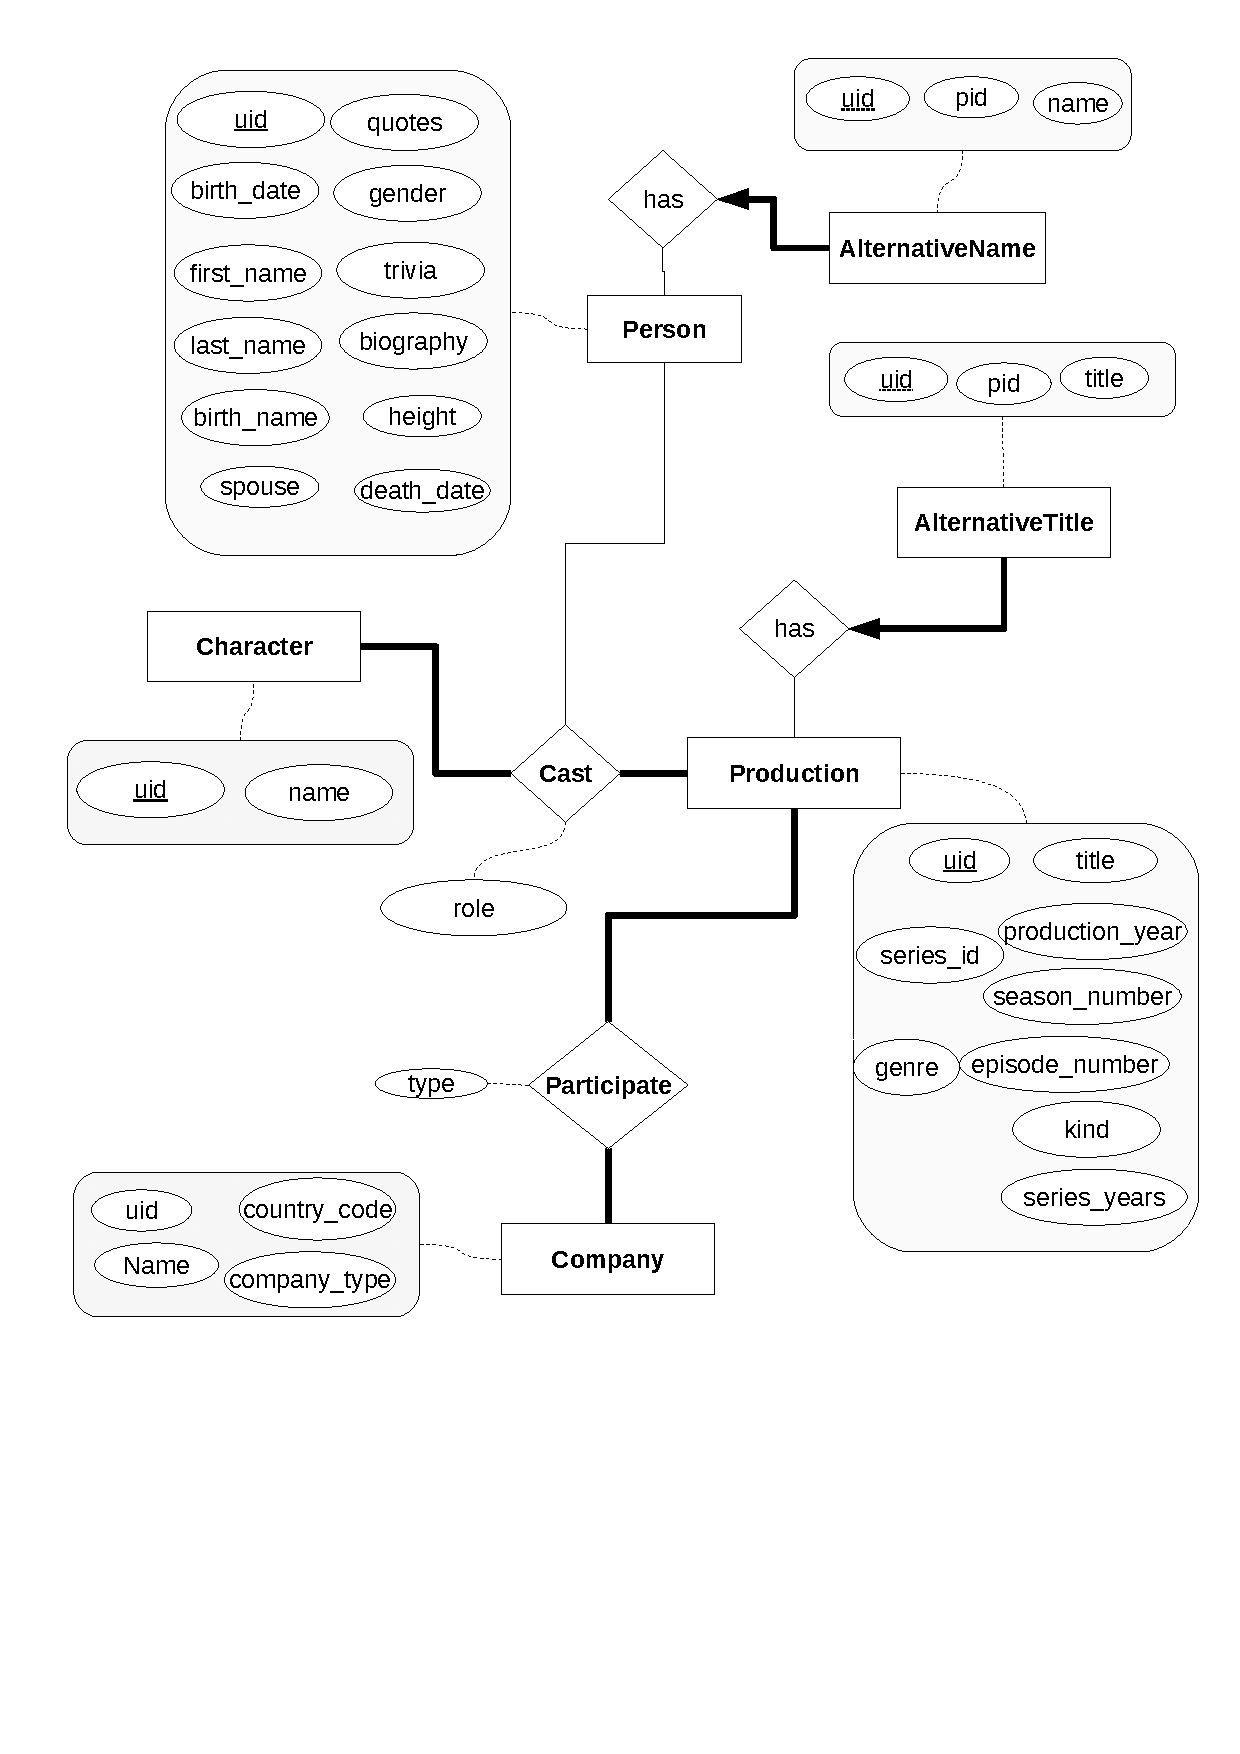
\includegraphics[width=\linewidth]{Diagrame_ER.pdf}
        \captionsetup{justification=centering}
        \caption{ER model of our DBMS}
    \end{figure}

\subsection{Table creation}
    We will implement the next deliverables using our own server with PostGreSQL.
    As such the types used in the following CREATE TABLE possibly doesn't work well in an
    Oracle DB environnement.
    \begin{lstlisting}[
           language=SQL,
           showspaces=false,
           basicstyle=\ttfamily,
           autogobble=true,
           commentstyle=\color{gray}
        ]
    CREATE TABLE person
       (uid INTEGER NOT NULL,
        first_name CHAR(75) NOT NULL,
        last_name CHAR(75) NOT NULL,
        gender CHAR(1),
        trivia TEXT,
        quotes VARCHAR(4000),
        birth DATE,
        death DATE,
        biography TEXT,
        spouse CHAR(100),
        height DOUBLE PRECISION,
        primary key (uid));

    CREATE TABLE alternative_name
       (uid INTEGER NOT NULL,
        pid INTEGER NOT NULL,
        name CHAR(60) NOT NULL,
        primary key (uid),
        foreign key (pid) references person(uid)
        ON DELETE CASCADE);
    
    CREATE TABLE character
       (uid INTEGER NOT NULL,
        name CHAR(60) NOT NULL,
        primary key (uid));
    
    CREATE TYPE CAST_ROLE AS
        ENUM ('actor', 'actress', 'producer', 'writer', 'cinematographer',
        'composer', 'costume designer', 'director', 'editor', 'miscellaneous crew',
        'production designer');
    
    CREATE TABLE production
       (uid INTEGER NOT NULL,
        title CHAR(80) NOT NULL,
        production_year DATE,
        genre CHAR(20),
        primary key (uid));
    
    CREATE TABLE casting
       (cid INTEGER,
        perid INTEGER NOT NULL,
        prodid INTEGER NOT NULL,
        role CAST_ROLE NOT NULL,
        primary key (cid, perid, prodid, role),
        foreign key (cid) references character (uid),
        foreign key (perid) references person (uid),
        foreign key (prodid) references production (uid));
    
    
    CREATE TABLE tv_serie
       (series_years CHAR(11),
        primary key (uid)) INHERITS (Production);
    
    CREATE TABLE episode
       (sid INTEGER NOT NULL,
        season SMALLINT NOT NULL,
        episode SMALLINT NOT NULL,
        primary key (uid),
        foreign key (sid) references tv_serie (uid)
        ON DELETE CASCADE) INHERITS (production);
    
    CREATE TABLE tv_movie
        (primary key (uid)) INHERITS (production);
    
    CREATE TABLE movie
        (primary key (uid)) INHERITS (production);
    
    CREATE TABLE video_movie
        (primary key (uid)) INHERITS (production);
    
    CREATE TABLE video_game
        (primary key (uid)) INHERITS (production);
    
    CREATE TYPE COMPANY_TYPE AS ENUM ('distributors', 'production company');
    
    CREATE TABLE company
       (uid INTEGER NOT NULL,
        name CHAR(80) NOT NULL,
        country_code CHAR(6),
        primary key (uid));
    
    CREATE TABLE participate
       (pid INTEGER NOT NULL,
        cid INTEGER NOT NULL,
        type COMPANY_TYPE NOT NULL,
        primary key (pid, cid),
        foreign key (pid) references production(uid),
        foreign key (cid) references company(uid));
    
    CREATE TABLE alternative_title
       (uid INTEGER NOT NULL,
        pid INTEGER NOT NULL,
        title CHAR (80) NOT NULL,
        primary key (uid),
        foreign key (pid) references production (uid)
        ON DELETE CASCADE);
    \end{lstlisting}

\pagebreak
\subsection{Discussion about constraint}
    A person can have one or more alternative name but an alternative name can describe only one person. We thus have a one-to-many relationship set. Also if the person is deleted from the database, his alternative names (if any) will be too. We thus created a weak entity for alternative name.
    We applied the same design choice for two similar situations: the production and its alternative title(s) and the tv serie and its episode(s). \\
    
    A production cast make the connection between the production, the person and the character (if any). We thus made a ternary relationship between the three entity person, character and production. We add the role of the person as an attribute of the relationship set. A character exist only if related to at least one person and one production. The person and production entity don't have this constraint since a production can have only a director that won't have any character.  \\
    
    Companies can be involved into production. They can play roles of different type (for example production, distribution), thus we added an attribute to the relationship "participate" called type instead of having a lot of duplicated entries in the "Company" table. Since that design choice, the data set given has been changed and comforted us in our design choice as the "type" attribute has been moved out of the COMPANY.csv file. A production need to have at least one company involved.\\
    
    We used enums for both the company type and the cast role because their value options are limited. As such we'll avoid repeating a considerable amount of bytes between the many lines sharing the same value for that field.\\
    
    And last but not least, instead of having a huge melting pot table called production, we made a "parent table" with all the fields shared between the different kinds of production and then we have a table per production kind which inherit from the production table and where some kind have additional info such as the season number in episode. This is the implementation of an IS A relationship in PostGreSQL. This allow us again to avoid having many entries of a table with some null field that they'd never have a value for.

\pagebreak
\section{Second deliverable}

\subsection{First deliverable changes}
    Since deliverable one we had to do several change on the table creation queries.
    First of all, the casting table now has its own index as it is indeed not correct to have a nullable element in a primary key! (its type is serial and its value is set automatically!
    Second of all, the PostGreSQL inheritance dream turned sour when we found out that this functionnality works perfectly by itself, as we described it. But you can't have a foreign key pointing to that parent table to reference everything including child table.
    As such, we were forced to get rid of the inheritance, as we need a foreign key for productions, both in $alternative\_title$ and $casting$!
    Also, we got rid of most $CHAR(some\_int)$ for $TEXT$ because there is often one or two values that are much longer that the others and if you use a $CHAR()$ you'd have to allocate bytes to fit the longest entry for each line even the shorter. With $TEXT$ the allocation is more clever and the number of bytes for a field is variable between lines. This change reduced greatly the size of our database tables. 
    Eventually, we added the field "birth name" to the person table which we forgot to add for the first deliverable. 
    Here are the new table creation instructions as a recap.
    \begin{lstlisting}[
           language=SQL,
           showspaces=false,
           basicstyle=\ttfamily,
           autogobble=true,
           commentstyle=\color{gray}
        ]
CREATE TABLE person
   (uid INTEGER NOT NULL,
    first_name TEXT,
    last_name TEXT NOT NULL,
    gender CHAR(1),
    trivia TEXT,
    quotes TEXT,
    birth DATE,
    death DATE,
    biography TEXT,
    spouse TEXT,
    height DOUBLE PRECISION,
    birth_name TEXT,
    primary key (uid));

CREATE TABLE alternative_name
   (uid INTEGER NOT NULL,
    pid INTEGER NOT NULL,
    name TEXT NOT NULL,
    primary key (uid),
    foreign key (pid) references person(uid)
    ON DELETE CASCADE);

CREATE TABLE character
   (uid INTEGER NOT NULL,
    name TEXT NOT NULL,
    primary key (uid));

CREATE TYPE CAST_ROLE AS
    ENUM ('actor', 'actress', 'producer', 'writer', 'cinematographer',
    'composer', 'costume designer', 'director', 'editor', 'miscellaneous crew',
    'production designer');

CREATE TYPE PRODUCTION_KIND AS
    ENUM ('tv series', 'episode', 'movie', 'video movie',
    'tv movie', 'video game');

CREATE TABLE production
   (uid INTEGER NOT NULL,
    title TEXT NOT NULL,
    production_year INT,
    kind PRODUCTION_KIND,
    genre CHAR(20),
    primary key (uid));

CREATE TABLE casting
   (uid SERIAL,
    cid INTEGER,
    perid INTEGER NOT NULL,
    prodid INTEGER NOT NULL,
    role CAST_ROLE NOT NULL,
    primary key (uid),
    foreign key (cid) references character (uid),
    foreign key (perid) references person (uid),
    foreign key (prodid) references production (uid));


CREATE TABLE tv_series
   (uid INTEGER NOT NULL,
    series_years CHAR(10),
    primary key (uid),
    foreign key (uid) references production (uid));

CREATE TABLE episode
   (uid INTEGER NOT NULL,
    sid INTEGER NOT NULL,
    season SMALLINT,
    episode INTEGER,
    primary key (uid),
    foreign key (uid) references production (uid),
    foreign key (sid) references tv_serie (uid)
    ON DELETE CASCADE);

CREATE TYPE COMPANY_TYPE AS ENUM ('distributors', 'production companies');

CREATE TABLE company
   (uid INTEGER NOT NULL,
    country_code CHAR(6),
    name TEXT NOT NULL,
    primary key (uid));

CREATE TABLE participate
   (uid INTEGER NOT NULL,
    pid INTEGER NOT NULL,
    cid INTEGER NOT NULL,
    type COMPANY_TYPE NOT NULL,
    primary key (uid),
    foreign key (pid) references production(uid),
    foreign key (cid) references company(uid));

CREATE TABLE alternative_title
   (uid INTEGER NOT NULL,
    pid INTEGER NOT NULL,
    title TEXT NOT NULL,
    primary key (uid),
    foreign key (pid) references production (uid)
    ON DELETE CASCADE);
    \end{lstlisting}


\subsection{SQL queries}
Here are the specific queries required in the 2nd deliverable specifications.

A) Number of movies per production year
    \begin{lstlisting}[
           language=SQL,
           showspaces=false,
           basicstyle=\ttfamily,
           autogobble=true,
           commentstyle=\color{gray}
        ]
        
    SELECT production_year, COUNT(*) FROM production
    WHERE (kind = 'movie'
        OR kind = 'tv movie'
        OR kind = 'video movie')
        AND production_year IS NOT NULL
    GROUP BY production_year
    ORDER BY production_year ASC;
    \end{lstlisting}
\medskip

B) Top 10 countries with the most production companies
    \begin{lstlisting}[
           language=SQL,
           showspaces=false,
           basicstyle=\ttfamily,
           autogobble=true,
           commentstyle=\color{gray}
        ]

    SELECT c.country_code, COUNT(DISTINCT c.uid) AS count 
    FROM company c
    LEFT JOIN participate par ON c.uid = par.cid
    WHERE par.type = 'production companies'
        AND c.country_code IS NOT NULL
    GROUP BY c.country_code
    ORDER BY count DESC LIMIT 10;
    \end{lstlisting}
    
\medskip

C) Compute the min, max and average career duration
    \begin{lstlisting}[
           language=SQL,
           showspaces=false,
           basicstyle=\ttfamily,
           autogobble=true,
           commentstyle=\color{gray}
        ]
        
    SELECT avg(duration) AS avg_duration, MAX(duration) AS max_duration, 
    MIN(duration) AS min_duration
    FROM (  
        SELECT (1+(MAX(prod.production_year)-MIN(prod.production_year))) 
        AS duration
        FROM casting c, production prod
        WHERE c.prodid = prod.uid
        GROUP BY c.perid
        ) AS career_duration;
    \end{lstlisting}
\medskip

D) Compute the min, max and average number of actors in a production
    \begin{lstlisting}[
           language=SQL,
           showspaces=false,
           basicstyle=\ttfamily,
           autogobble=true,
           commentstyle=\color{gray}
        ]
        
    SELECT avg(numb) AS avg_nb_act, MAX(numb) AS max_nb_act, 
    MIN(numb) AS min_nb_act
    FROM (  SELECT count(*) AS numb
            FROM casting
            WHERE role = 'actor'
            GROUP BY prodid
    ) AS number;
    \end{lstlisting}
\medskip

E) Min, Max, Avg height of female persons
    \begin{lstlisting}[
           language=SQL,
           showspaces=false,
           basicstyle=\ttfamily,
           autogobble=true,
           commentstyle=\color{gray}
        ]
        
    SELECT MIN(height) AS min_height, MAX(height) AS max_height, 
    AVG(height) AS avg_height 
    FROM person
    WHERE gender = 'f';
    \end{lstlisting}
\medskip

F) List all pairs of persons and movies where the person has both directed the movie and acted in the movie. Do not include tv and videos movies
    \begin{lstlisting}[
           language=SQL,
           showspaces=false,
           basicstyle=\ttfamily,
           autogobble=true,
           commentstyle=\color{gray}
        ]
        
    SELECT p2.uid, p1.uid, person.first_name, person.last_name, 
    prod.title, p1.role, p2.role 
    FROM casting p1
    LEFT JOIN casting p2 ON p1.prodid = p2.prodid AND p1.perid = p2.perid
    LEFT JOIN person ON p1.perid = person.uid
    LEFT JOIN production prod ON p1.prodid = prod.uid
    WHERE p1.role='director' AND p2.role='actor';
    \end{lstlisting}
\medskip

G) List the three most popular character names
    \begin{lstlisting}[
           language=SQL,
           showspaces=false,
           basicstyle=\ttfamily,
           autogobble=true,
           commentstyle=\color{gray}
        ]
        
    SELECT name, COUNT(*) AS amount
    FROM character
    GROUP BY name
    ORDER BY amount DESC LIMIT 3;
    \end{lstlisting}
\medskip

\subsection{Index Creation}
In order to increase our queries execution speed (which are relatively long as the server hosting our PostGreSQL database is only running a intel Atom D2500!) we created indexes on all foreign key fields in our tables.
And, in addition to that we also created an index on $role$ in casting, $last\_name$ and $gender$ in person, $production\_year$, $genre$ and $kind$ in production and $country\_code$ in company.

Here is one of the create index instructions:
\begin{lstlisting}[
           language=SQL,
           showspaces=false,
           basicstyle=\ttfamily,
           autogobble=true,
           commentstyle=\color{gray}
        ]
        
    CREATE INDEX CONCURRENTLY casting_perid_index ON casting(perid);
    \end{lstlisting}

\subsection{Graphical User Interface Design}

For the method to apply on a graphical user interface (GUI) allowing to query our movie database, we choose an opensource internet framework written in python, Django \footnote{Django Software Fondation, https://www.djangoproject.com} (preset queries where implemented with a pyscopg2 query but the keyword search is implemented with django Models system, but we're using the raw() function which allows us to write SQL normally for the request!). The graphical design was focused on giving an open space to the user rather than a high-density function in a unique window.\\

\begin{figure}[H]
        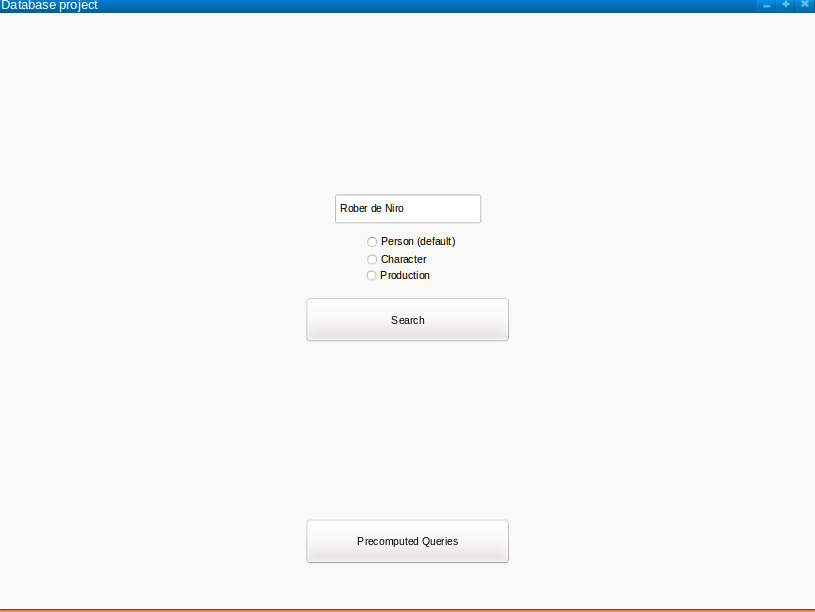
\includegraphics[width=\linewidth]{mainpage.png}
        \captionsetup{justification=centering}
        \caption{Main page v0.12}
    \end{figure}

Based on that, we design a main window with only the general search, meaning a text entry, a validation button and three radioboxes to specified what kind of search the user intend to do : by person, by movie or by casting. Once the user made a search, the results are display in a form of a list summarizing the informations retrieved from the database. The result window keeps the three general search components in case the user would want to adapt his search. We also add the possibility to recieve further informations on a part of the result by cliquing on it, this will in fact run a search query base on the type of the object of the user interest.\\

\begin{figure}[H]
        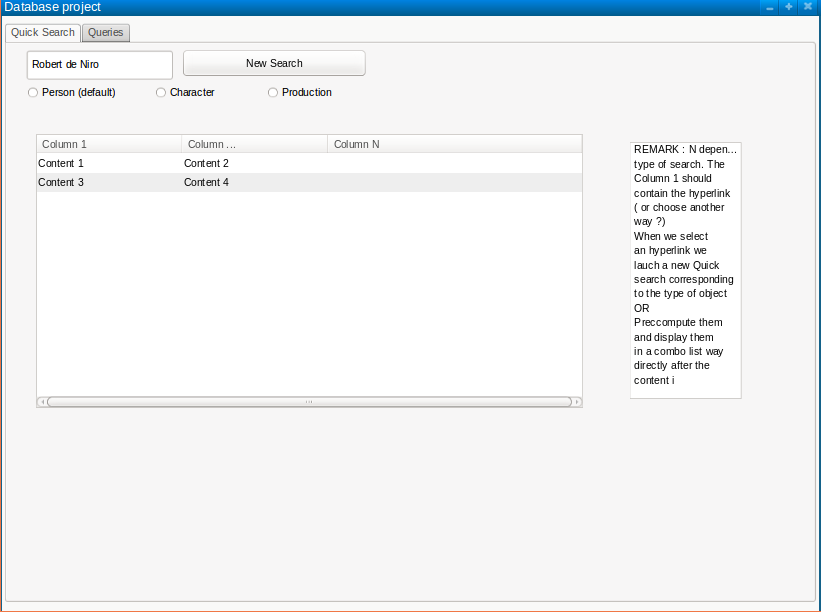
\includegraphics[width=\linewidth]{result_quick.png}
        \captionsetup{justification=centering}
        \caption{Result of the keyword search v0.12}
    \end{figure}

Then, to display the deliverable queries and their results, we used a menu list (comparable to an onglet system) to switch from the general search (default window) to the list of the deliverable queries (at the end 21 queries). Also here clicking on one component of this list will trigger the associated SQL query and display the results in a new window to easily adapt the layout of the results. Indeed, the kind of results may diverge greatly from a unique row to several hundreds of them.
\begin{figure}[H]
        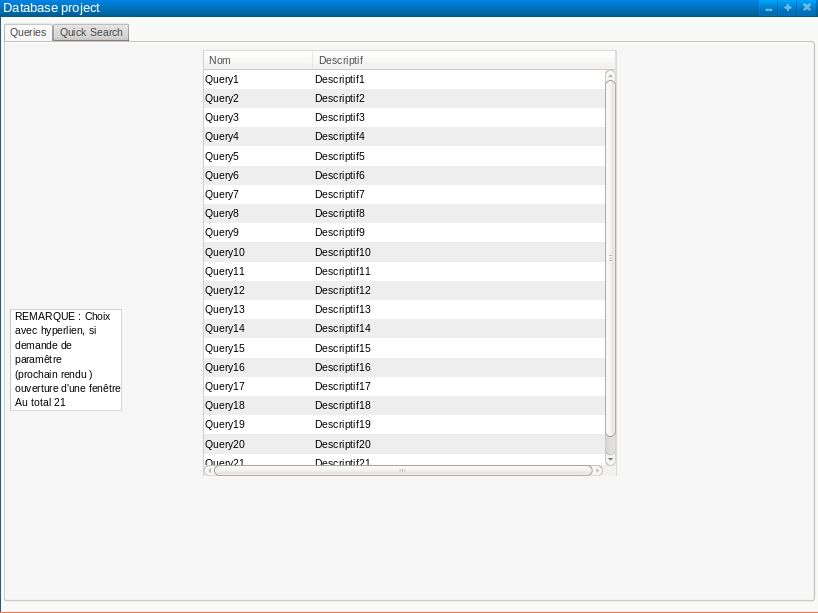
\includegraphics[width=\linewidth]{preset_list.png}
        \captionsetup{justification=centering}
        \caption{List of the preset queries v0.12}
    \end{figure}
%************************************THIRD*DELIVERABLE*********************************
\section{Third deliverable}

\subsection{SQL queries}

A)\\
SELECT DISTINCT p1.uid as person_id, c1.prodid as production_id\\
FROM person p1\\
LEFT JOIN casting c1 ON p1.uid = c1.perid\\
LEFT JOIN casting c2 ON c1.prodid = c2.prodid\\
LEFT JOIN person p2 ON c2.perid = p2.uid\\
WHERE (p1.birth IS NOT NULL AND p2.birth IS NOT NULL AND p1.uid <> p2.uid AND p1.birth >= p2.birth + 55 * interval '1 year') \\
OR (p1.birth IS NOT NULL AND p2.birth IS NOT NULL AND p1.uid <> p2.uid AND p1.birth >= p2.birth + 55 * interval '1 year' )\\
OR (p1.birth IS NOT NULL AND p2.birth IS NOT NULL AND p1.uid <> p2.uid AND p1.birth >= p2.birth + 55 * interval '1 year' )\\
OR (p1.birth IS NOT NULL AND p2.birth IS NOT NULL AND p1.uid <> p2.uid AND p1.birth >= p2.birth + 55 * interval '1 year');\\

B)\\
SELECT production_year\\
FROM (\\
	SELECT production_year, COUNT(*) AS count\\
	FROM ( SELECT production_year\\
		FROM person\\
		LEFT JOIN casting ON person.uid = casting.perid \\
		LEFT JOIN production ON casting.prodid = production.uid\\
		WHERE last_name = 'Cooper' AND first_name = 'Bradley'\\
		) AS prod_year\\
	GROUP BY production_year\\
	ORDER BY count DESC LIMIT 1\\
	) AS year;\\

C)\\
(SELECT genre, name, count(*) as nombre_de_prod\\
FROM participate pa\\
LEFT JOIN production p ON pa.pid = p.uid\\
LEFT JOIN company c ON pa.cid = c.uid\\
WHERE production_year = 2000 AND p.genre = 'Action'\\  
GROUP BY name, genre\\
ORDER BY nombre_de_prod DESC LIMIT 1)\\
UNION \\
(SELECT genre, name, count(*) as nombre_de_prod\\
FROM participate pa\\
LEFT JOIN production p ON pa.pid = p.uid\\
LEFT JOIN company c ON pa.cid = c.uid\\
WHERE production_year = 2000 AND p.genre = 'Adventure' \\ 
GROUP BY name, genre\\
ORDER BY nombre_de_prod DESC LIMIT 1)\\
UNION\\
(SELECT genre, name, count(*) as nombre_de_prod\\
FROM participate pa\\
LEFT JOIN production p ON pa.pid = p.uid\\
LEFT JOIN company c ON pa.cid = c.uid\\
WHERE production_year = 2000 AND p.genre = 'Animation'  \\
GROUP BY name, genre\\
ORDER BY nombre_de_prod DESC LIMIT 1)\\
UNION\\
(SELECT genre, name, count(*) as nombre_de_prod\\
FROM participate pa\\
LEFT JOIN production p ON pa.pid = p.uid\\
LEFT JOIN company c ON pa.cid = c.uid\\
WHERE production_year = 2000 AND p.genre = 'Biography'  \\
GROUP BY name, genre\\
ORDER BY nombre_de_prod DESC LIMIT 1)\\
UNION \\
(SELECT genre, name, count(*) as nombre_de_prod\\
FROM participate pa\\
LEFT JOIN production p ON pa.pid = p.uid\\
LEFT JOIN company c ON pa.cid = c.uid\\
WHERE production_year = 2000 AND p.genre = 'Comedy'\\  
GROUP BY name, genre\\
ORDER BY nombre_de_prod DESC LIMIT 1)\\
UNION\\
(SELECT genre, name, count(*) as nombre_de_prod\\
FROM participate pa\\
LEFT JOIN production p ON pa.pid = p.uid\\
LEFT JOIN company c ON pa.cid = c.uid\\
WHERE production_year = 2000 AND p.genre = 'Crime'  \\
GROUP BY name, genre\\
ORDER BY nombre_de_prod DESC LIMIT 1)\\
UNION\\
(SELECT genre, name, count(*) as nombre_de_prod\\
FROM participate pa\\
LEFT JOIN production p ON pa.pid = p.uid\\
LEFT JOIN company c ON pa.cid = c.uid\\
WHERE production_year = 2000 AND p.genre = 'Documentary'\\  
GROUP BY name, genre\\
ORDER BY nombre_de_prod DESC LIMIT 1)\\
UNION \\
(SELECT genre, name, count(*) as nombre_de_prod\\
FROM participate pa\\
LEFT JOIN production p ON pa.pid = p.uid\\
LEFT JOIN company c ON pa.cid = c.uid\\
WHERE production_year = 2000 AND p.genre = 'Drama'  \\
GROUP BY name, genre\\
ORDER BY nombre_de_prod DESC LIMIT 1)\\
UNION\\
(SELECT genre, name, count(*) as nombre_de_prod\\
FROM participate pa\\
LEFT JOIN production p ON pa.pid = p.uid\\
LEFT JOIN company c ON pa.cid = c.uid\\
WHERE production_year = 2000 AND p.genre = 'Family'  \\
GROUP BY name, genre\\
ORDER BY nombre_de_prod DESC LIMIT 1)\\
UNION\\
(SELECT genre, name, count(*) as nombre_de_prod\\
FROM participate pa\\
LEFT JOIN production p ON pa.pid = p.uid\\
LEFT JOIN company c ON pa.cid = c.uid\\
WHERE production_year = 2000 AND p.genre = 'Fantasy'  \\
GROUP BY name, genre\\
ORDER BY nombre_de_prod DESC LIMIT 1)\\
UNION \\
(SELECT genre, name, count(*) as nombre_de_prod\\
FROM participate pa\\
LEFT JOIN production p ON pa.pid = p.uid\\
LEFT JOIN company c ON pa.cid = c.uid\\
WHERE production_year = 2000 AND p.genre = 'Film-Noir'  \\
GROUP BY name, genre\\
ORDER BY nombre_de_prod DESC LIMIT 1)\\
UNION\\
(SELECT genre, name, count(*) as nombre_de_prod\\
FROM participate pa\\
LEFT JOIN production p ON pa.pid = p.uid\\
LEFT JOIN company c ON pa.cid = c.uid\\
WHERE production_year = 2000 AND p.genre = 'Game-Show'  \\
GROUP BY name, genre\\
ORDER BY nombre_de_prod DESC LIMIT 1)\\
UNION\\
(SELECT genre, name, count(*) as nombre_de_prod\\
FROM participate pa\\
LEFT JOIN production p ON pa.pid = p.uid\\
LEFT JOIN company c ON pa.cid = c.uid\\
WHERE production_year = 2000 AND p.genre = 'History'  \\
GROUP BY name, genre\\
ORDER BY nombre_de_prod DESC LIMIT 1)\\
UNION \\
(SELECT genre, name, count(*) as nombre_de_prod\\
FROM participate pa\\
LEFT JOIN production p ON pa.pid = p.uid\\
LEFT JOIN company c ON pa.cid = c.uid\\
WHERE production_year = 2000 AND p.genre = 'Horror'\\  
GROUP BY name, genre\\
ORDER BY nombre_de_prod DESC LIMIT 1)\\
UNION\\
(SELECT genre, name, count(*) as nombre_de_prod\\
FROM participate pa\\
LEFT JOIN production p ON pa.pid = p.uid\\
LEFT JOIN company c ON pa.cid = c.uid\\
WHERE production_year = 2000 AND p.genre = 'Music'  \\
GROUP BY name, genre\\
ORDER BY nombre_de_prod DESC LIMIT 1)\\
UNION\\
(SELECT genre, name, count(*) as nombre_de_prod\\
FROM participate pa\\
LEFT JOIN production p ON pa.pid = p.uid\\
LEFT JOIN company c ON pa.cid = c.uid\\
WHERE production_year = 2000 AND p.genre = 'Musical' \\ 
GROUP BY name, genre\\
ORDER BY nombre_de_prod DESC LIMIT 1)\\
UNION \\
(SELECT genre, name, count(*) as nombre_de_prod\\
FROM participate pa\\
LEFT JOIN production p ON pa.pid = p.uid\\
LEFT JOIN company c ON pa.cid = c.uid\\
WHERE production_year = 2000 AND p.genre = 'Mystery'  \\
GROUP BY name, genre\\
ORDER BY nombre_de_prod DESC LIMIT 1)\\
UNION\\
(SELECT genre, name, count(*) as nombre_de_prod\\
FROM participate pa\\
LEFT JOIN production p ON pa.pid = p.uid\\
LEFT JOIN company c ON pa.cid = c.uid\\
WHERE production_year = 2000 AND p.genre = 'News'\\  
GROUP BY name, genre\\
ORDER BY nombre_de_prod DESC LIMIT 1)\\
UNION\\
(SELECT genre, name, count(*) as nombre_de_prod\\
FROM participate pa\\
LEFT JOIN production p ON pa.pid = p.uid\\
LEFT JOIN company c ON pa.cid = c.uid\\
WHERE production_year = 2000 AND p.genre = 'Reality-TV'  \\
GROUP BY name, genre\\
ORDER BY nombre_de_prod DESC LIMIT 1)\\
UNION \\
(SELECT genre, name, count(*) as nombre_de_prod\\
FROM participate pa\\
LEFT JOIN production p ON pa.pid = p.uid\\
LEFT JOIN company c ON pa.cid = c.uid\\
WHERE production_year = 2000 AND p.genre = 'Romance'\\  
GROUP BY name, genre\\
ORDER BY nombre_de_prod DESC LIMIT 1)\\
UNION\\
(SELECT genre, name, count(*) as nombre_de_prod\\
FROM participate pa\\
LEFT JOIN production p ON pa.pid = p.uid\\
LEFT JOIN company c ON pa.cid = c.uid\\
WHERE production_year = 2000 AND p.genre = 'Sci-Fi'  \\
GROUP BY name, genre\\
ORDER BY nombre_de_prod DESC LIMIT 1)\\
UNION\\
(SELECT genre, name, count(*) as nombre_de_prod\\
FROM participate pa\\
LEFT JOIN production p ON pa.pid = p.uid\\
LEFT JOIN company c ON pa.cid = c.uid\\
WHERE production_year = 2000 AND p.genre = 'Short'  \\
GROUP BY name, genre\\
ORDER BY nombre_de_prod DESC LIMIT 1)\\
UNION \\
(SELECT genre, name, count(*) as nombre_de_prod\\
FROM participate pa\\
LEFT JOIN production p ON pa.pid = p.uid\\
LEFT JOIN company c ON pa.cid = c.uid\\
WHERE production_year = 2000 AND p.genre = 'Sport'  \\
GROUP BY name, genre\\
ORDER BY nombre_de_prod DESC LIMIT 1)\\
UNION\\
(SELECT genre, name, count(*) as nombre_de_prod\\
FROM participate pa\\
LEFT JOIN production p ON pa.pid = p.uid\\
LEFT JOIN company c ON pa.cid = c.uid\\
WHERE production_year = 2000 AND p.genre = 'Talk-Show'\\  
GROUP BY name, genre\\
ORDER BY nombre_de_prod DESC LIMIT 1)\\
UNION\\
(SELECT genre, name, count(*) as nombre_de_prod\\
FROM participate pa\\
LEFT JOIN production p ON pa.pid = p.uid\\
LEFT JOIN company c ON pa.cid = c.uid\\
WHERE production_year = 2000 AND p.genre = 'Thriller'\\  
GROUP BY name, genre\\
ORDER BY nombre_de_prod DESC LIMIT 1)\\
UNION \\
(SELECT genre, name, count(*) as nombre_de_prod\\
FROM participate pa\\
LEFT JOIN production p ON pa.pid = p.uid\\
LEFT JOIN company c ON pa.cid = c.uid\\
WHERE production_year = 2000 AND p.genre = 'War' \\ 
GROUP BY name, genre\\
ORDER BY nombre_de_prod DESC LIMIT 1)\\
UNION\\
(SELECT genre, name, count(*) as nombre_de_prod\\
FROM participate pa\\
LEFT JOIN production p ON pa.pid = p.uid\\
LEFT JOIN company c ON pa.cid = c.uid\\
WHERE production_year = 2000 AND p.genre = 'Western'\\  
GROUP BY name, genre\\
ORDER BY nombre_de_prod DESC LIMIT 1)\\

D)\\
SELECT c1.prodid, p1.last_name, p1.first_name, p2.last_name, p2.first_name\\
FROM casting c1\\
LEFT JOIN person p1 ON c1.perid = p1.uid\\
LEFT JOIN casting c2 ON c1.prodid = c2.prodid\\
LEFT JOIN person p2 ON c2.perid = p2.uid\\
WHERE p1.uid <> p2.uid AND p1.last_name = p2.last_name ;\\

E)\\
SELECT p.production_year, COUNT(*) / COUNT(DISTINCT p.uid)\\
FROM casting c\\
LEFT JOIN production p ON c.prodid = p.uid\\
WHERE c.role = 'actor' OR c.role = 'actress'\\ 
GROUP BY p.production_year\\
ORDER BY p.production_year;\\

F)\\
SELECT AVG(num) \\
FROM (	SELECT COUNT(*) AS num\\
	FROM episode\\
	GROUP BY sid, season\\
	) AS nb_episode;\\

G)\\
SELECT AVG (numb) \\
FROM 	(SELECT count(DISTINCT season) AS numb\\
	FROM episode\\
	GROUP BY sid\\
	) AS count;\\

H)\\
SELECT p.title, COUNT( DISTINCT e.season ) AS nb_seasons\\
FROM episode AS e, production AS p\\
WHERE p.uid = e.sid AND p.kind = 'tv series'\\
GROUP BY p.uid\\
ORDER BY nb_seasons DESC\\
LIMIT 10 ;\\

I)\\
SELECT p.title,\\ 
(count(e.episode) / CASE COUNT( DISTINCT e.season ) WHEN 0 THEN 1 ELSE COUNT( DISTINCT e.season ) END) AS nb_episode_p_season\\
FROM episode AS e\\
INNER JOIN production AS p ON p.uid = e.sid AND p.kind = 'tv series'\\
GROUP BY p.uid\\
ORDER BY nb_episode_p_season DESC\\
LIMIT 10 ;\\

J)\\
SELECT per.first_name, per.last_name, per.death \\
FROM person As per\\
LEFT OUTER JOIN casting AS c ON (per.uid = c.perid AND per.death IS NOT NULL)\\
LEFT OUTER JOIN production AS prod ON (prod.uid = c.prodid)\\
WHERE (prod.production_year > EXTRACT( YEAR FROM per.death) AND c.role = 'actor' ) OR\\
	(prod.production_year > EXTRACT( YEAR FROM per.death) AND c.role = 'actress' ) OR\\
(prod.production_year > EXTRACT( YEAR FROM per.death) AND c.role = 'director');\\

K)\\
SELECT DISTINCT production_year AS year, comp.name, num_movie, Rank\\
FROM(\\
    SELECT DISTINCT *, RANK() OVER (PARTITION BY production_year ORDER BY num_movie DESC) AS Rank\\
    FROM (\\
        SELECT part.cid, prod.production_year, COUNT(*) AS num_movie\\
        FROM production AS prod\\
        JOIN participate AS part ON prod.uid = part.pid\\
        WHERE prod.production_year IS NOT NULL\\
        GROUP BY part.cid, prod.production_year\\
    ) AS MoviesPerCompanyInAYear\\
) AS MoviesPerCompanyInAYearWithRank\\
JOIN company AS comp ON comp.uid = cid\\
WHERE Rank <= 3\\
ORDER BY production_year, num_movie DESC;\\

L)\\
SELECT first_name, last_name, DATE_PART('year',NOW())-DATE_PART('year', birth) AS age\\
FROM person\\
WHERE (biography LIKE '% opera singer %' AND death IS NULL) OR\\
(trivia LIKE '% opera singer %' AND death IS NULL)\\
ORDER BY age ASC ;\\

M)\\
SELECT prod.title, prod.production_year, per.first_name, per.last_name, prod.nb_alias * per.nb_alias AS deg_ambig\\
FROM\\
(\\
	SELECT per.uid, per.first_name, per.last_name, count(*)+1 as nb_alias\\
	FROM person AS per\\
	INNER JOIN alternative_name AS a_name ON a_name.pid = per.uid\\
	GROUP BY per.uid\\
) AS per,\\
(\\
	SELECT prod.uid, prod.title, prod.production_year, count(*)+1 as nb_alias\\
	FROM production AS prod\\
	INNER JOIN alternative_title AS a_title ON prod.uid = a_title.pid\\
	GROUP BY prod.uid\\
) AS prod\\
WHERE EXISTS (\\ 
	SELECT *\\
	FROM casting AS cas\\
	WHERE cas.prodid = prod.uid AND cas.perid = per.uid\\
)\\
ORDER BY deg_ambig DESC\\
LIMIT 10 ;\\

N)\\
SELECT  country_code, name, name_tot\\
FROM(\\
    SELECT DISTINCT *, RANK() OVER (PARTITION BY country_code ORDER BY name_tot DESC) AS rank\\
    FROM (\\
        SELECT DISTINCT comp.country_code, char.name, COUNT(*) AS name_tot\\
       FROM company as comp\\
	JOIN participate as part ON part.cid=comp.uid AND part.type= 'production company'\\
	JOIN production as prod ON prod.uid = part.pid\\
	JOIN casting AS cas ON prod.uid = cas.prodid\\
	JOIN character AS char ON char.uid = cas.cid\\
        WHERE comp.country_code IS NOT NULL\\
        GROUP BY comp.country_code, char.name\\
    ) AS NameWithNameCountPerCountry\\
) AS NameWithNameCountPerCountryWithRank\\
WHERE rank <= 1\\
ORDER BY country_code ASC;\\

\subsection{Query plan, index utility and cost distribution}

For the present and following sections we have choosen three queries, the B), J) and .\\

B) Query plan \\
"Subquery Scan on year  (cost=1709.10..1709.11 rows=1 width=4) (actual time=7.375..7.377 rows=1 loops=1)"\\
"  ->  Limit  (cost=1709.10..1709.10 rows=1 width=4) (actual time=7.373..7.373 rows=1 loops=1)"\\
"        ->  Sort  (cost=1709.10..1709.12 rows=7 width=4) (actual time=7.371..7.371 rows=1 loops=1)"\\
"              Sort Key: (count(*))"\\
"              Sort Method: top-N heapsort  Memory: 25kB"\\
"              ->  HashAggregate  (cost=1708.99..1709.06 rows=7 width=4) (actual time=7.208..7.231 rows=41 loops=1)"\\
"                    Group Key: production.production_year"\\
"                    ->  Nested Loop Left Join  (cost=1.43..1708.96 rows=7 width=4) (actual time=0.189..6.733 rows=187 loops=1)"\\
"                          ->  Nested Loop Left Join  (cost=1.00..1705.72 rows=7 width=4) (actual time=0.155..0.905 rows=187 loops=1)"\\
"                                ->  Index Scan using person_lastname_index on person  (cost=0.43..469.82 rows=1 width=4) (actual time=0.108..0.351 rows=2 loops=1)"\\
"                                      Index Cond: (last_name = 'Reno'::text)"\\
"                                      Filter: (first_name = 'Jean'::text)"\\
"                                      Rows Removed by Filter: 126"\\
"                                ->  Index Scan using casting_perid_index on casting  (cost=0.56..1230.14 rows=576 width=8) (actual time=0.036..0.192 rows=94 loops=2)"\\
"                                      Index Cond: (person.uid = perid)"\\
"                          ->  Index Scan using production_uid_index on production  (cost=0.43..0.45 rows=1 width=8) (actual time=0.026..0.028 rows=1 loops=187)"\\
"                                Index Cond: (casting.prodid = uid)"\\
"Planning time: 6.776 ms"\\
"Execution time: 8.074 ms"\\

Three indexes were used in this query: person_lastname_index, casting_perid_index and production_uid_index.\\

The index on person.last_name is used in the WHERE clause. Index scan is used to find the rows matching the index condition <last_name = 'Damon'>. Fetching the table rows in index order make them more expensive to read but there are so few that at the end it lower the reading cost. \\

The "first_name" clause is applied as a filter on the rows retrieved by the index. Using a second index on "first_name" wasn't necessary since there was few output row from the first clause. It would have been more expensive to visit both index. \\

Then the index on casting.perid and on production.uid are used in the inner index scan of both LEFT JOIN clause. The use of index nested loop is best when having one relation is small and the other indexed. This is the case here:
\begin{itemize}
\item \<person.uid = casting.perid\> : the resulted rows of person.uid are few because of the WHERE clause and there is an index on casting.perid.\\
\item \<casting.prodid> = production.uid : the resulted rows of casting.prodid are few because of the resulting left join and there is an index on production.uid. \\
\end{itemize}

J) Query plan \\
 Nested Loop  (cost=117340.56..1455804.06 rows=60763 width=17)\\
   Join Filter: ((prod.production_year)::double precision > date_part('year'::text, (per.death)::timestamp without time zone))\\
   ->  Hash Join  (cost=117340.13..1368053.03 rows=182290 width=21)\\
         Hash Cond: (c.perid = per.uid)\\
         ->  Seq Scan on casting c  (cost=0.00..1029263.28 rows=21962672 width=8)\\
               Filter: ((role = 'actor'::cast_role) OR (role = 'actress'::cast_role) OR (role = 'director'::cast_role))\\
         ->  Hash  (cost=116700.22..116700.22 rows=51193 width=21)\\
               ->  Seq Scan on person per  (cost=0.00..116700.22 rows=51193 width=21)\\
                     Filter: (death IS NOT NULL)\\
   ->  Index Scan using production_uid_index on production prod  (cost=0.43..0.46 rows=1 width=8)\\
         Index Cond: (uid = c.prodid)\\
(11 rows)\\

Time: 5.659 ms\\

Only one index is used by postgres in this query : production_uid_index. But several others indexes could used in the joins : casting_prodid_index,  casting_role_index,casting_perid_index. But postgres used sequencial scan on the join's conditions.\\

The index on the production.uid is used to efficiently join casting and production accoriding to his id. The other side of the join equality can't use both indexes, so a sequential scan of all entry in the table is made.\\

The distribution of the cost is almost the same for the nested loop, the hash Join and the Hash. Of course the sequential scan has a variable cost from zero to the cost of the operation calling it (hash and hash join). Those costs are very high because of the complexity of a tow large table join.\\







\end{document}
